\section{PAGRINDINIAI DIMENSIJŲ ATRINKIMO METODAI}

Biomedicininių duomenų kontekste galima daryti prielaidą, kad ne visi matai yra susiję su tiriama problema, pvz. gaubtinės žarnos vėžiu, dėl tokių faktorių, kaip triukšmas duomenyse. Paprastai nagrinėjamai problemai svarbus yra mažas, palyginus su visu, matų kiekis. Ši biomedicininių duomenų ypatybė veda prie ,,daugiamatiškumo prakeiksmo`` (angl. \textit{the curse of dimentionality}) \cite{bellman1966adaptive} - didėjant matų kiekiui mėginiai pasidaro panašūs, todėl bandymas juos klasifikuoti tolygus spėliojimui. Vienas iš būdų kovoti su ,,daugiamatiškumo prakeiksmu`` yra naudoti dimensijų atrinkimo metodus. Dimensijų atrinkimas yra svarbus etapas biomedicininių duomenų pirminiam apdorojimui (angl. \textit{preprocessing}). Dimensijų atrinkimas dažniausiai yra naudojamas surasti mažiausią dimensijų poaibį, kuris maksimaliai pagerina klasifikatoriaus tikslumą.

Pagal tai, kaip dimensijų atrinkimo metodai yra susiję su klasifikatoriumi, dimensijų atrinkimo metodus galima skirstyti į tris kategorijas \cite{saeys2008robust}:
\begin{enumerate}
 \item Filtruojantys metodai (angl. \textit{filter methods}), pvz. \textit{Fisher} įvertis. Jie dirba tiesiogiai su duomenimis, o jų rezultatas gali būti dimensijų įvertinimas svoriais, dimensijų reitingavimas ar tiesiog geriausių dimensijų poaibis, kuriuo remiantis vėliau apmokomas klasifikatorius. Tokių metodų pagrindinis privalumas yra tai, kad jie yra greiti, tinka paskirstytų skaičiavimų aplinkoms ir nepriklausomi nuo klasifikavimo  metodo, tačiau remiantis atrinktosiomis dimensijomis nebūtinai bus sukurtas geriausias klasifikatorius.
 \item Prisitaikantieji metodai (angl. \textit{wrapper methods}). Pirma, apmokomas klasifikatorius su visomis dimensijomis, antra, parenkamas dimensijų poaibis ir apmokomas klasifikatorius, tada po daugkartinio dimensijų aibių įvertinimo pagal klasifikavimo rezultatus yra nusprendžiama, kuris dimensijų poaibis yra labiausiai tinkamas klasifikavimui. Įterptinių metodų atveju dimensijų atrinkimo procesas yra neatsiejamas nuo klasifikavimo proceso - pats klasifikatorius įvertina dimensijas. Jie dažnai duoda geresnius rezultatus negu filtravimo metodai, bet yra reiklūs resursams.
 \item Įterptiniai metodai (angl. \textit{embedded methods}), pvz. AW-SVM\cite{vapnik2000nature}. Jie dimensijų atrinkimui naudoja vidinius klasifikatoriaus duomenis (pvz. dimensijų svoriai gauti pagal SVM). Šie metodai dažnai siūlo gerą santykį tarp klasifikavimo tikslumo ir skaičiavimų sudėtingumo.
\end{enumerate}

Šiame skyriuje nagrinėsiu pagrindinius dimensijų atsirinkimo metodus:
\begin{enumerate}
 \item \textit{Fisher} įvertis (angl. \textit{Fisher ratio})\cite{Pavlidis:2001:GFC:369133.369228};
 \item \textit{Relief} metodas\cite{DBLP:journals/ml/Robnik-SikonjaK03};
 \item Asimetrinis priklausomybės koeficientas\cite{Shannon:2001:MTC:584091.584093} (angl. \textit{Asymmetric Dependency Coefficient, ADC});
 \item Absoliučių svorių SVM\cite{vapnik2000nature} (AW-SVM) (angl. \textit{Absolute Weight SVM})
 \item Rekursyvus dimensijų eliminavimas pagal SVM\cite{Guyon:2002:GSC:599613.599671} (SVM-RFE) (angl. \textit{Recursive Feature Elimination by SVM})
\end{enumerate}

\subsection{\textit{Fisher} įvertis}

\textit{Fisher} įvertis vertina individualias dimensijas pagal dimensijos klasių atskiriamąją galią. Dimensijos įvertis yra sudarytas iš tarpklasinio skirtumo santykio su vidiniu klasės pasiskirstymu:
\begin{equation}
 FR(j) = \frac{(\mu_{j1} - \mu_{j2})^2}{\sigma_{j1}^2 + \sigma_{j2}^2},
\end{equation}
kur, 
$j$ - yra dimensijos indeksas, 
$\mu_{jc}$ - dimensijos $j$ reikšmių vidurkis klasėje $c$, 
$\sigma_{jc}^2$ - dimensijos $j$ reikšmių standartinis nuokrypis klasėje $c$, kur $c={1,2}$. Kuo didesnis yra \textit{Fisher} įvertis, tuo geriau ta dimensija atskiria klases.

\subsection{\textit{Relief} metodas}

\textit{Relief} metodas iteratyviai skaičiuoja dimensijų ,,susietumą``. Pradžioje
,,susietumas`` visoms dimensijoms yra lygus nuliui. Kiekvienoje
iteracijoje atsitiktinai\footnote{Pastebėtina, kad dėl atsitiktinumo faktoriaus klasifikavimo ir  dimensijų atrinkimo stabilumo
rezultatai varijuoja.} pasirenkamas objektas iš mėginių aibės, surandami
artimiausi kaimynai iš tos pačios ir kitos klasės, ir atnaujinamos visų 
dimensijų ,,susietumo`` reikšmės. Dimensijos įvertis yra vidurkis visų objektų
atstumų iki artimiausių kaimynų iš tos pačios ir kitos klasės:
\begin{equation}
 W(j)=W(j) - \frac{diff(j, x, x_H)}{n} + \frac{diff(i, x, x_M)}{n},
\end{equation}
kur 
$W(j)$ - $j$-osios dimensijos ,,susietumo`` įvertis, 
$n$ - mėginių aibės dydis, 
$x$ - atsitiktinai pasirinktas mėginys, 
$x_H$ - artimiausias $x$ kaimynas iš tos pačios klasės (angl. \textit{nearest-Hit}), 
$x_M$ - artimiausias $x$ kaimynas iš kitos klasės(angl. \textit{nearest-Miss}),
$diff(j, x, x')$ - $j$-osios dimensijos reikšmių skirtumas tarp laisvai pasirinkto objekto $x$ ir atitinkamo kaimyno, kur skirtumą į intervalą $[0, 1]$ normalizuojanti funkcija yra:
\begin{equation}
 diff(j, x, x')=\frac{|x_j- x_j'|}{x_{j_{max}} - x_{i_{min}}},
\end{equation}
kur $x_{j_{max}}$ ir $x_{j_{min}}$ yra maximali ir minimali $j$-osios dimensijos reikšmės. ,,Susietumo`` reikšmių atnaujinimas yra vykdomas $n$ kartų ir kuo didesnė galutinė reikšmė, tuo svarbesnė dimensija. Pastebėtina, kad aprašyta algoritma versija yra skirta dirbti su dviejų klasių atveju, tačiau yra ir multiklasinis algoritmo variantas.

\subsection{Asimetrinis priklausomybės koeficientas}

Asimetrinis priklausomybės koeficientas (ADC) yra dimensijų reitingavimo motodas, kuris matuoja klasės $Y$ etiketės (angl. \textit{label}) tikimybinę priklausomybę $j$-ąjai dimensijai, naudodamas informacijos prieaugį \cite{kent1983information} (angl. information gain):
\begin{equation}
 ADC(Y, j) = \frac{MI(Y, X_j)}{H(Y)},
\end{equation}
kur $H(Y)$ - klasės $Y$ entropija \cite{Shannon:2001:MTC:584091.584093}, o $MI(Y, X_j)$ - yra bendrumo informacija \cite{Shannon:2001:MTC:584091.584093} (angl. mutual information) tarp klasės etiketės $Y$ ir $j$-osios dimensijos
\begin{equation}
 H(Y)=-\sum_y{p(Y=y)log{p(Y=y)}}, 
\end{equation}
\begin{equation}
 H(X_j)=-\sum_x{p(X_j=x) log{p(X_j=x)}},
\end{equation}
\begin{equation}
 MI(Y, X_j) = H(Y) + H(X_j) - H(Y, X_j),
\end{equation}
\begin{equation}
 H(Y, X_j) = -\sum_{y,x_j}{p(y, x_j)log{p(y, x_j)}},
\end{equation}
Kuo didesni ADC įverčiai, tuo dimensija yra svarbesnė, nes turi daugiau informacijos apie mėginių klases.

\subsection{Absoliučių svorių SVM}

Atraminių vektorių metodas (SVM) yra vienas populiariausių klasifikavimo algortimų, nes jis gerai susidoroja su daugiamačiais duomenimis \cite{guyon2002gene}. Yra keletas bazinių SVM variantų \cite{vapnik2000nature}, bet šiame darbe naudosime tiesinį SVM, nes jis demonstruoja gerus rezultatus analizuojant genų ekspresijos duomenimis. Tiesinis SVM yra hiperplokštuma apibrėžta kaip:
\begin{equation}
 \sum_{j=1}^{p}{w_jx_j + b_0 = 0},
\end{equation}
kur $p$ - dimensijų kiekis, $w_j$ - j-osios dimensijos svoris, $x_j$ - j-osios
dimensijos kintamasis, $b_0$ - konstanta. Dimensijos absoliutus\footnote{Svorį
reikia imti absoliutaus dydžio, nes neigiamas svoris implikuoja priklausomybę 
vienai klasei, o teigiamas kitai klasei.} svoris $w_j$ gali būti panaudotas
dimensijų reitingavimui. Pastebėtina, kad svorių nustatymas yra atliekamas tik 
vieną kartą\footnote{SVM-RFE dimensijų atrinkimo metodas svorius nustato daug kartų.}.

\subsection{Rekursyvus dimensijų eliminavimas pagal SVM}

Rekursyvus dimensijų eliminavimas pagal SVM \cite{guyon2002gene} yra vienas populiariausių dimensijų
atrinkimo algoritmų. Todėl, jis yra naudojamas, kaip atskaitos taškas (angl. \textit{benchmark})
vertinant kitus dimensijų atrankos metodus. Iš esmės šis metodas yra daugkartinis 
absoliučių svorių SVM metodo taikymas nuolat išmetinėjant dimensijas su 
mažiausiais svoriais. Rekursyvus dimensijų eliminavimas mums padeda surasti 
tinkamą dimensijų poaibį, kas nevisada pavyksta su dimensijų reitingavimo 
metodais. Bendroji rekursyvaus dimensijų eliminavimo procedūra:
\begin{algorithm}
\caption{Rekursyvus dimensijų eliminavimas}
\label{RFE}
 \begin{enumerate}
 \item Turime pilną dimensijų rinkinį $F_0$, nustatome $i=0$;
 \item Įvertiname kiekvienos dimensijos kokybę dimensijų aibėje $F_i$;
 \item Išmetame mažiausiai kokybišką dimensiją iš $F_I$ tam, kad gautume
 dimensijų rinkinį $F_{i+1}$;
 \item Nustatome $i=i+1$ ir grįžtame į antrąjį žingsnį kol nėra patenkinta 
 algoritmo pabaigos sąlyga.
\end{enumerate}
\end{algorithm}
Jei trečiajame algoritmo žingsnyje iš dimensijų aibės yra pašalinama tik viena dimensija, tai gauname dimensijų reitingavimą, o jei pašalinamas fiksuotas skaičius ar dalis (pvz. 50\%) dimensijų, tai dimensijų reitingavimo negauname. Pastebėtina, kad rekursyvus dimensijų eliminavimas labai padidina algoritmo sudėtingumą. Algoritmo pabaigos sąlyga gali būti koks nors konkretus dimensijų skaičius arba tiesiog dimensijų aibę mažinti tol, kol dimensijų visai nebeliks.

\section{STABILIŲ DIMENSIJŲ ATRINKIMO METODAI}
\label{stabiliu_dimensiju_atrinkimo_metodai}

Naudodami dimensijų atrinkimo metodus, biomedicininius duomenis tiriantys mokslininkai susiduria su atrinktųjų dimensijų aibės stabilumo problema - atrenkant dimensijas pagal kitą mėginių poaibį, gaunamas kitas dimensijų poaibis. Dimensijų atrinkimo nestabilumas yra sąlygotas šių veiksnių:
\begin{enumerate}
 \item Duomenys yra triukšmingi ir kai kurios dimensijos gali būti palaikytos informatyviomis grynai dėl atsitiktinių priežasčių;
 \item Daugiamačiuose duomenyse tikėtina, kad dalis dimensijų koreliuoja, todėl, kuri iš koreliuojančių dimensijų bus pasirinkta, priklauso nuo to, kuriuos mėginius pasirinksime klasifikatoriaus apmokymui;
 \item Kiekvienas dimensijų atrinkimo algoritmas daro skirtingas prielaidas apie tai, kurios dimensijos yra informatyvios.
\end{enumerate}
Galime teigti, kad skirtingi metodai tiems patiems duomenims gali atrinkti skirtingas dimensijas. Taip pat, suskaidžius turimus duomenis į atskiras persidengiančias aibes ir atrinkus tą patį kiekį dimensijų tuo pačiu metodu, gaunamos skirtingos dimensijų aibės. Be to, kuo triukšmingesni duomenys, kuo mažiau turima mėginių ir kuo daugiau yra dimensijų, tuo ryškesnė yra ši problema \cite{loscalzo2009consensus}. 

Vienas iš būdų didinti dimensijų atrinkimo stabilumą yra naudoti multikriterinius dimensijų atrinkimo metodus. Jų esmė yra panaudoti kelis dimensijų atrinkimo metodus suliejant jų rezultatus į vieną bendrą rezultatą. Yra skiriamos trys priežastys, kodėl keletas agreguotų silpnų ir nestabilių dimensijų atrinkimo metodų gali duoti stabilesnius dimensijų atrinkimo rezultatus \cite{dietterich2000ensemble}:
\begin{enumerate}
 \item Keletas skirtingų, bet vienodai optimalių hipotezių gali būti teisingos, ir kriterijų agregavimas sumažiną tikimybę, kad bus pasirinkta neteisinga  hipotezė;
 \item Atskiri dimensijų metodai gali dirbti skirtinguose lokaliuose optimumuose, tuo tarpu agregavimas gali geriau reprezentuoti tikrąją  duomenis generuojančią funkciją;
 \item Tikroji duomenų funkcija negali būti reprezentuojama jokia hipoteze paskiro algoritmo hipotezių erdvėje ir agreguojant pavienių metodų rezultatus galima praplėsti hipotezių erdvę.
\end{enumerate}
Apibendrinant galima sakyti, kad suliejant keletą skirtingų dimensijų atrinkimo metodų rezultatų suliejamos gerosios pavienių dimensijų atrinkimo metodų savybės, taip bandant kompensuoti tų algoritmų silpnybes.

Šiame skyriuje aptarsiu dimensijų atrinkimo stabilumą didinančius metodus:
\begin{enumerate}
 \item Svoriais grįstas multikriterinis suliejimas;
 \item Reitingais grįstas multikriterinis suliejimas;
 \item Svoriais ir reitingais grįstas multikriterinis suliejimas;
 \item Multikriterinis rekursyvus dimensijų eliminavimas;
 \item Konsensuso grupėmis grįstas stabilių dimensijų atrinkimo metodas.
\end{enumerate}

\subsection{Svoriais grįstas multikriterinis suliejimas}

Svoriais grįsto multikriterinio dimensijų atrinkimo suliejimo pagal svorius algoritmo
pirmajame žingsnyje kiekvienas bazinis metodas priskiria duomenų rinkinio
dimensijoms svorius, tada tie svoriai yra kombinuojami į vieną sutarties
(angl. consensus) svorių vektorių, kurio pagrindu yra gaunami dimensijų 
reitingai. Algoritmas yra pavaizduotas ~\ref{fig:figure4} pav.
\begin{figure}
 \centering
 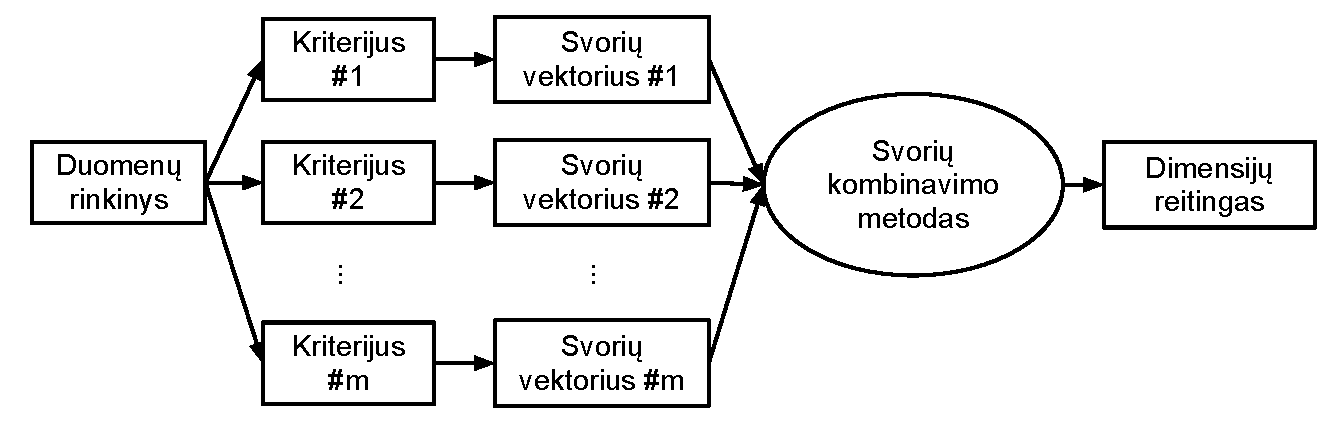
\includegraphics[width=1\textwidth]{images/score_based_fusion.pdf}
 \caption{Svoriais grįstas multikriterinis suliejimas.}
 \label{fig:figure4}
\end{figure}
\begin{figure}[ht]
\begin{minipage}[b]{0.5\linewidth}
\centering
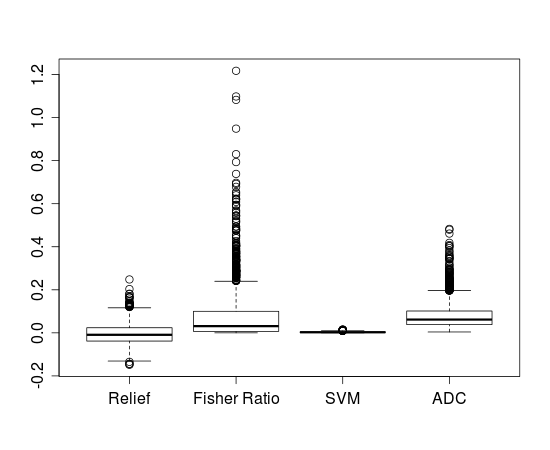
\includegraphics[width=1\textwidth]{images/boxplot_colon_all.png}
\caption{Pavienių dimensijų atrinkimo metodų nenormalizuotas svorių
pasiskirstymas.}
\label{fig:figure1}
\end{minipage}
\hspace{0.5cm}
\begin{minipage}[b]{0.5\linewidth}
\centering
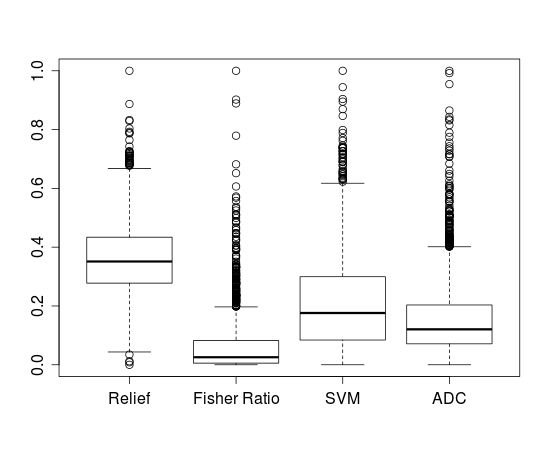
\includegraphics[width=1\textwidth]{images/boxplot_colon_all_normalized.png}
\caption{Pavienių dimensijų atrinkimo metodų normalizuotas svorių
pasiskirstymas.}
\label{fig:figure2}
\end{minipage}
\end{figure}

Suliejant svorius svarbu yra užtikrinti, kad svoriai, gauti naudojant
skirtingus bazinius kriterijus, būtų palyginami. Todėl svorių normalizavimas
turi būti atliekamas prieš svorių kombinavimą. Kitu
atveju dimensijų įvertinimo metodai bus nepalyginami. Paveikslėlyje ~\ref{fig:figure1} pav.
nenormalizuotų pavienių dimensijų vertinimo metodų skiriasi netgi suteiktų
svorių intervalai. Paveikslėlyje ~\ref{fig:figure2} pav. matome,
kad net ir normalizavus svorius gana stipriai skiriasi svorių kvartiliai - į 
tai reikia atkreipti dėmesį interpretuojant galutinius dimensijų vertinimo 
rezultatus. Šiame darbe svoriai yra 
normalizuoti intervale $[0, 1]$ pagal formulę:
\begin{equation}
 u_i'=\frac{u_i - u_{i_{min}}}{u_{i_{max}} - u_{i_{min}}}, 
\end{equation}
kur $u_i$ - dimensijų svorių vektorius pagal $i$ kriterijų, 
$u_{i_{min}}$ - minimali $u_i$ svorių vektoriaus reikšmė,
$u_{i_{max}}$ - maksimali $u_i$ svorių vektoriaus reikšmė,
$u_i'$ - normalizuotų svorių vektorius.

Sutarties svorių vektorius $u$ yra vidurkis normalizuotų svorių vektorių:
\begin{equation}
 u = \frac{1}{m}\sum_{i=1}^m u_i',
\end{equation}
kur $m$ yra bazinių kriterijų skaičius. Reikia paminėti, kad didesnė svorio
reikšmė reiškia, kad dimensija yra geresnė.

\subsection{Reitingais grįstas multikriterinis suliejimas}

Reitingais grįsto multikriterinio suliejimo pagal reitingus metodas gauna
duomenų rinkinio dimensijų reitingą,
pagal keletą bazinių dimensijų reitingavimo kriterijų. Algoritmo pirmajame žingsnyje
keletas dimensijų atrinkimo kriterijų grąžina dimensijų reitingu, paskui tie
reitingai yra kombinuojami į vieną bendra dimensijų reitingą.  Algoritmas yra
pavaizduotas ~\ref{fig:figure5} pav.
\begin{figure}
 \centering
 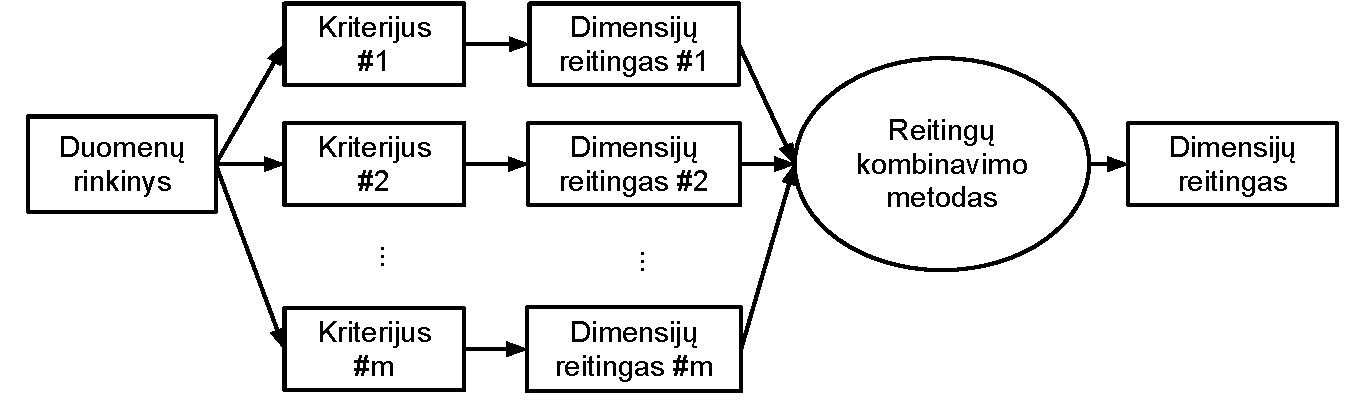
\includegraphics[width=1\textwidth]{images/ranking_based_fusion.pdf}
 \caption{Reitingais grįstas multikriterinis suliejimas.}
 \label{fig:figure5}
\end{figure}
Suliejimo pagal reitingus metodas nereikalauja dimensijų atrinkimo metodų 
rezultatų normalizavimo, nes tiesiog imame dimensijoms priskirtus reitingus ir 
juos kombinuojame. Skirtingai nei suliejimo pagal svorius algoritme, baziniai 
dimensijų atrinkimo kriterija dimensijų eliminavimas\cite{yang2011robust} susideda iš dviejų
dalių: keletos dimensijų atrinkimi turi gražinti dimensijų reitingus, o ne svorius.

Dimensijų reitingų kombinavimui yra keletas metodų\cite{dwork2001rank}, tačiau
paprastumo dėlei šiame darbe naudosiu Borda balsavimą\footnote{Dar žinomas kaip
,,Pažymių metodas``. Jis buvo pasiūlytas prancūzų matematiko ir fiziko 
Jean-Charles de Borda 1770 metais.} (angl. Borda count). Tarkime, kad turime
$m$ basuotojų ir $p$ kandidatų aibę. Tada Borda balsavimo metodas kiekvienam
$i$-ajam balsuotojui sukuria balsų vektorių $v_i$ tokiu būdu: geriausiai 
įvertintam kandidatui suteikiama $p$ taškų, antrajam kandidatui $p-1$, ir t.t.
Galutiniai taškai yra gaunami sudedant visų balsuotojų taškus
\begin{equation}
 v = \sum_{i=1}^m v_i,
\end{equation}
kur $v$ yra suminių taškų vektorius, o iš jo galime gauti ir dimensijų reitingus.

\subsection{Svoriais ir reitingais grįstas multikriterinis suliejimas}

Svoriais ir reitingais grįsto multikriterinio suliejimo metodas
nuo reitingais grįsto multikriterinio suliejimo metodo skiriasi tuo, kad kaip dar vienas 
reitingas yra panaudojamas svoriais grįsto multikriterinio dimensijų atrinkimo metu
gautas reitingas.
Multikriterinio dimensijų įverčių ir pagal svorius, ir pagal reitingus metodas vyksta trimis
žingsniais:
\begin{enumerate}
  \item Gauname dimensijų reitingus pagal $m$ pavienių dimensijų atrinkimo motodų;
  \item Suliejame dimensijų įverčius pagal svorius ir taip gauname vieną 
  dimensijų reitingą;
  \item Reitinguojame dimensijas pagal visus turimus $m+1$ pavienius reitingus.
\end{enumerate} 
Algoritmas yra pavaizduotas ~\ref{fig:figure3} pav.
\begin{figure}
 \centering
 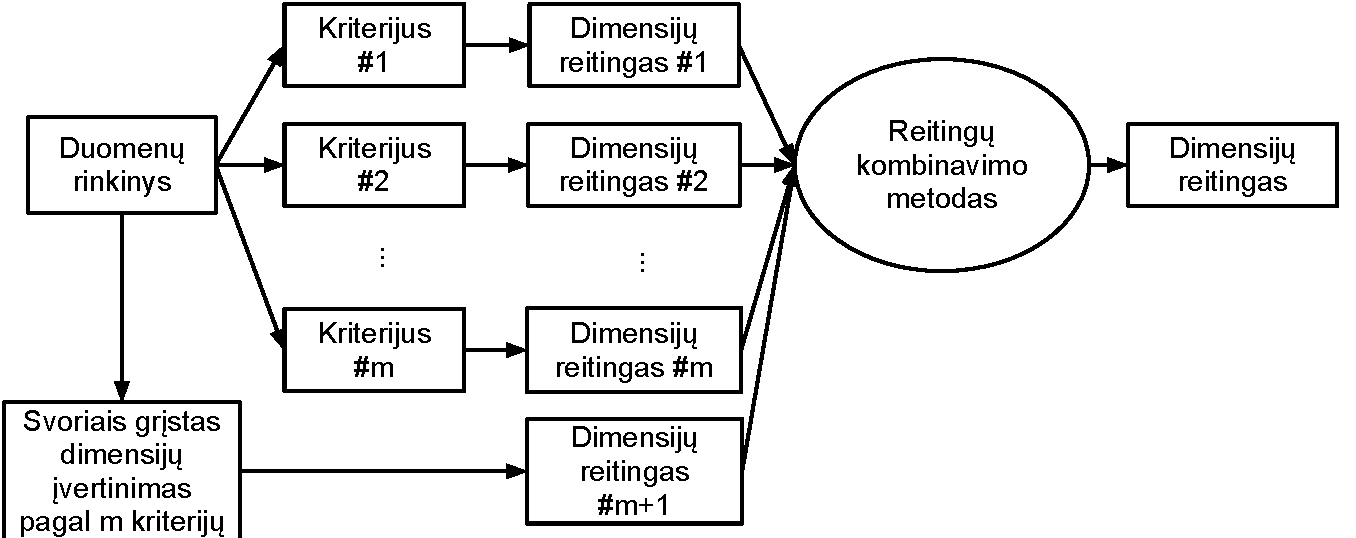
\includegraphics[width=1\textwidth]{images/score_and_ranking_based_fusion.pdf}
 \caption{Svoriais ir reitingais grįstas multikriterinis suliejimas.}
 \label{fig:figure3}
\end{figure}

Kadangi yra suliejami keli mažai koreliuojantys dimensijų reitingavimo metodai,
yra pasiekiamas didesnis dimensijų atrinkimo stabilumas, kai varijuoja 
treniravimosi duomenų poaibis (angl. subsampling).

\subsection{Multikriterinis rekursyvus dimensijų eliminavimas}

Jei dimensijų atrinkimo tikslas yra pagerinti klasifikavimo rezultatus, tai taikymas
multikriterinio dimensijų atrinkimo metodų nebūtinai duos pageidaujamą rezultatą,
nes yra pastebėta, kad vien dimensijų reitingavimas nebūtinai suranda geriausią dimensijų 
poaibį. Tam, kad būtų surastas geriausias dimensijų poaibis reikia kombinuoti
multikriterinį dimensijų reitingavimą su paieškos strategija. Rekursyvus 
dimensijų eliminavimas yra dažnai naudojama paieškos strategija dimensijų
atrinkimui. Todėl yra kombinuojamas multikriterinis dimensijų reitingavimas ir
rekursyvus dimensijų eliminavimas.

Multikriterinis rekursyvus dimensijų eliminavimas\cite{yang2011robust} susideda iš dviejų
dalių: keletos dimensijų atrinkimo kriterijų suliejimo ir pagal svorius, ir 
pagal reitingus, ir rekursyvaus dimensijų eliminavimo aprašyto algoritme 
nr. \ref{RFE}. Algoritmas pavaizduotas ~\ref{fig:figure6} pav.
\begin{figure}
 \centering
 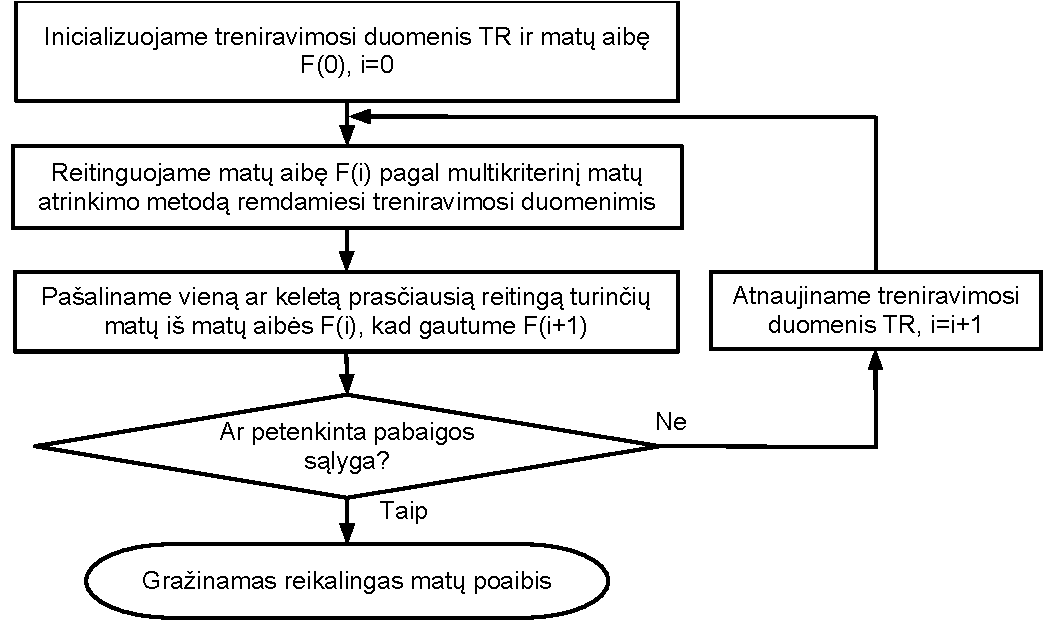
\includegraphics[width=0.7\textwidth]{images/mcf-rfe_procedure.pdf}
 \caption{Multikriterinio rekursyvaus dimensijų eliminavimo algoritmas.}
 \label{fig:figure6}
\end{figure}

Yra pastebėta, kad standartinis rekursyvus dimensijų eliminavimas, kai vienos
iteracijos metu yra eliminuojama viena dimensija, gali labai padidinti 
algoritmo sudėtingumą. Todėl genų ekspresijos duomenims yra rekomenduotina
eliminuoti keletą dimensijų vienu metu.

Nors SVM-RFE dimensijų atrinkimo algoritmas ir yra labai populiarus, tačiau yra
žinoma, kad jam trūksta stabilumo. Todėl kombinuodami didesnį stabilumą turintį
multikriterinį dimensijų atrinkimą su rekursyvaus dimensijų eliminavimo paieškos
strategija, turėtume gauti stabilesnį dimensijų atrinkimo algoritmą.

\subsection{Konsensuso grupėmis grįstas stabilių dimensijų atrinkimo metodas}

Konsensuso grupėmis grįstas stabilių dimensijų atrinkimo metodas\cite{loscalzo2009consensus}, pirma, identifikuoja panašių dimensijų grupes, antra, pagal surastas grupes transformuoja dimensijų erdvę, trečia, transformuotoje dimensijų erdvėje atlieka dimensijų atrinkimą. Schematiškai šis algoritmas pavaizduotas  ~\ref{fig:figure7} pav.

\begin{figure}
 \centering
 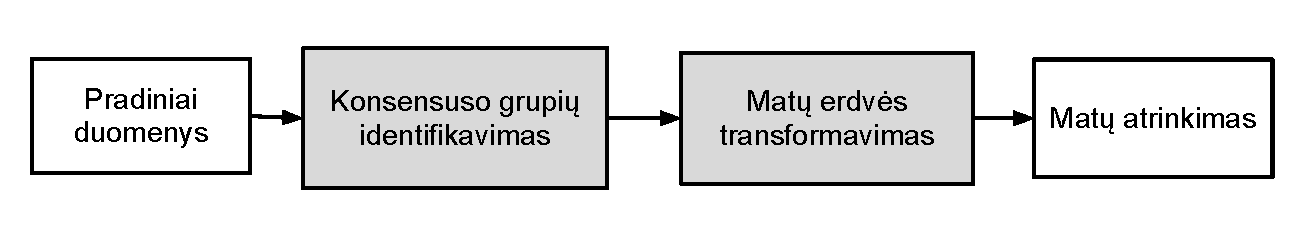
\includegraphics[width=\textwidth]{images/consensus_group_based_feature_selection_framework.pdf}
 \caption{Konsensuso grupėmis grįstas stabilių dimensijų atrinkimas.}
 \label{fig:figure7}
\end{figure}
Loscalzo pasiūlyto metodo pagrindinė dalis yra panašių dimensijų identifikavimas. Šio uždavinio sprendimui Loscalzo naudojo \textit{Dense Group Finder} (DGF) algoritmą. DGF aprašytas algoritme nr. \ref{DGF}.
\begin{algorithm}
\caption{DGF - \textit{Dense Group Finder}}
\label{DGF}
 \begin{algorithmic}
 \item \textbf{Įeitis:} duomenys $D=\{x_i\}_{i=1}^n$, branduolio plotis $h$
 \item \textbf{Išeitis:} tankios dimensijų grupės $G_1, G_1,..., G_L$
 \For{$i = 1$ \textbf{to} $n$ \do} 
  \State Inicializuojame $j=1, y_{i,j}=x_i$
  \Repeat
    \State Suskaičiuoti $y_{i, j+1}$ pagal (\ref{for_dgf})
  \Until{konverguoja}
  \State Nustatyti atskaitos tašką $y_{i,c} = y_{i,j+1}$ (Nustatyti piką $p_i$ kaip $y_{i,c}$)
  \State Sulieti piką $p_i$ su artimiausiais pikais jei atstumai tarp jų $ < h$
 \EndFor
 \item Iš kiekvieno unikalaus piko $p_r$, pridėkime $x_i$ į $G_r$ jei $||p_r - x_i|| < h$
 \end{algorithmic}
\end{algorithm}


\begin{equation}
\label{for_dgf}
  y_{i, j+1}=\frac{\sum_{i=1}^{n} x_i K(\frac{y_j - x_i}{h})}{\sum_{i=1}^{n} K(\frac{y_j - x_i}{h})} j=1,2,...
\end{equation}
kur

\begin{algorithm}
 \caption{Konsensuso grupėmis grįstas stabilių dimensijų atrinkimas}
 \label{CGS}
 \begin{algorithmic}
   \item \textbf{Įeitis:} mėginių aibė $D$, iteracijų skaičius $t$, dimensijų atrinkimo metodas $\Phi$\
   \item \textbf{Išeitis:} atrinktos konsensuso dimensijų grupės $CG_1, CG_1,..., CG_k$
   \item // Konsensuso grupių identifikavimas
   \For{$i = 1$ \textbf{to} $n$ \do}
    \State Parinkti mėginių  poaibį $D_i$ iš $D$
    \State Gauti tankių dimensijų grupes pagal $DGF(D_i, h)$
   \EndFor
   \For{kiekvienai dimensijų porai $X_i$ ir $X_j \in D$}
    \State Nustatyti $W_{i,j}=$ dažnis kai $X_i$ ir $X_j$ yra toje pačioje grupėje $/t$
   \EndFor
   \item Sudaryti konsensuso grupes $CG_1, CG_1,..., CG_L$ atliekant hierarchinį klasterizavimą visoms dimensijoms pagal $W_{i, j}$
   \item //Dimensijų atrinkimas grįstas konsensuso grupėmis
   \For{$i = 1$ \textbf{to} $l$ \do}
    \State Parinkti reprezentatyvią dimensiją $X_i$ iš $CG_i$
    \State Įvertinti dimensijos informatyvumą $\Phi(X_i)$
   \EndFor
   \item Reitinguoti konsensuso grupes $CG_1, CG_1,..., CG_L$ pagal $\Phi(X_i)$
   \item Pasirinkti $k$ dimensijų turinčių geriausią reitingą  
 \end{algorithmic}
\end{algorithm}
